\chapter{非线性差分方程的精确解与$n$阶展开方法}\label{ch04}
尽管线性多项式系数的差分方程并没有被完全解决, 但是它的解从多项式解开始变得越来越一般. 受该方程的解的发展过程的启发, 本文决定求解非线性多项式系数的差分方程的多项式解. 方程的形式为
\begin{equation}
\sum_{k=0}^l{\mbrace{a_k(x)\prod_{i=0}^r{f^{\gamma_{ki}}(x+i)}}}=0.
\label{eq}
\end{equation}
其中, $K$是一个数域, $a_k(x)\in K[x], l>1, \gamma_{ki}\ge 0$. 在本节中, 本文致力于寻找\refeqnn{eq}的多项式解. 

受到在微分受到在微分方程求解中被广泛应用的齐次平衡原则的启发, 本文用其求解非线性差分方程的多项式解. 齐次平衡原则通过平衡方程中最高次项的次数来确定解的次数, 只能在一些情况下生效. 本文考虑同时平衡方程中最高$n$项的次数和系数, 提出了$n$阶展开方法来处理齐次平衡原则不能处理的情况, 从而求得\refeqnn{eq}的多项式解. 

\section{齐次平衡原则与$n$阶展开方法}
设
\begin{equation}
f(x)=\sum_{k=0}^m{\mu_kx^k},
\label{fm1}
\end{equation}
将其代入\refeqn{eq}, 我们可以求得所有次数不超过$m$的多项式解. 为了求得方程的多项式解, 我们需要找到$m$的上界.

将\refeqn{fm1} 代入 \refeqn{eq}后, 方程的左端仍然是一个多项式, 这个多项式的各项次数为
\begin{equation}
D = \mbrace{s_1 m+d_1,s_2 m+d_2,\cdots,s_l m+d_l},
\end{equation}
其中
\begin{equation}
\begin{split}
s_k&=\sum_{i=0}^r{\gamma_{ki}}, \\
d_k&=\deg a_k(x).
\end{split}
\label{eq-sd}
\end{equation}
$D$ 中的每一个次数都是关于 $m$ 的线性表达式, 我们称其为该项的阶数.

方程的左端为零要求整理后的多项式的各项系数为零, 从而要求最高项的系数为零. 因为各个加法项的最高项系数非零, 所以至少有两个不同的最高项进行合并才能使得整理后的多项式最高项系数为零. 从而, 我们有 
\begin{equation}
\left\{
\begin{array}{l}
m\in \mathbb Z_+  ,                                     \\
\exists i\neq j, s_i m+d_i=s_j m+d_j    ,               \\
\forall k \not\in \bbrace{i,j}, s_i m+d_i\ge s_k m+d_k .
\end{array}
\right.
\label{cond}
\end{equation}
上式中的三个约束条件分别被称为: 整数性约束\D 平衡性约束和最大性约束. 

(I) 如果 $s_i \neq s_j$, 我们有 
\begin{equation}
m=\frac{d_j-d_i}{s_i-s_j}.
\end{equation}
如果$m$又同时满足\refeqn{cond}中的其它条件, 则我们称它为第一类平衡点(简称 \BPone{}). 第一类平衡点构成的集合为 
\begin{equation}
M_1=\bbrace{\left. m=\frac{d_j-d_i}{s_i-s_j}\in \mathbb Z_+\right\vert \forall k\not\in \bbrace{i,j}, s_i m+d_i\ge s_k m+d_k}.
\end{equation}

(II) 如果 $s_i = s_j, d_i=d_j$, 则能够始终满足平衡性约束. 考虑最大性约束, 我们有 
\begin{equation}
\left\{
\begin{split}
m > \frac{d_k-d_i}{s_i-s_k}, & \text{ if } s_i>s_k,  \\
m < \frac{d_k-d_i}{s_i-s_k}, & \text{ if } s_i<s_k.  \\
\end{split}
\right.
\end{equation}
因为\BPone{}的成立条件已经包含上述不等式中取等号的条件, 所以上述不等式不含等号. 求解上述不等式, 可以得到 
\begin{equation}
\underset{s_i>s_k}{\max}{\frac{d_k-d_i}{s_i-s_k}} < m < \underset{s_i<s_k}{\min}{\frac{d_k-d_i}{s_i-s_k}}.
\end{equation}
如果 $s_i m + d_i < \sigma m + \delta$, 则$m$存在上界. 这里, 
\begin{equation}
\begin{split}
\sigma &= \max ~s_k,  \\
\delta &= \underset{s_k=\sigma}{\max}{~d_k}.
\end{split}
\label{eq-max-sd}
\end{equation}

我们可以根$m$是否存在上界, 将剩下的情况细分为两种. 

(II-a) 当 $s_i m + d_i < \sigma m + \delta$时, $m$的取值范围有限. 我们可以得到第二类平衡点(简称 \BPtwo{}). 第二类平衡点构成的集合为
\begin{equation}
M_2=\bbrace{m\in \mathbb Z_+\left|\underset{s_i>s_k}{\max}{\frac{d_k-d_i}{s_i-s_k}} < m < \underset{s_i<s_k}{\min}{\frac{d_k-d_i}{s_i-s_k}}\right.} .
\end{equation}

(II-b) 当 $s_i m + d_i = \sigma m + \delta$ 时, 我们无法基于齐次平衡原则来确定$m$的上界. 因此, 我们提出了一个$n$阶展开方法来解决这个问题.

给定 $n>0$, 我们定义一个$m$次多项式的$n$阶展开多项式为
\begin{equation}
F\sbrace{x,m,u\up n}=\sum_{k=0}^{n-1}{u_k x^{m-k}}+\OO\sbrace{x^{m-n}},
\label{npoly}
\end{equation}
其中 $u\up n=\mbrace{u_0,u_1,\cdots,u_{n-1}}$是系数向量, 而
\begin{equation}
\OO\sbrace{x^n}=\left\{
\begin{array}{cl}
\text{次数不超过}\,n\,\text{的多项式} & n\ge 0, \\
0                                                 & n<0 .
\end{array}
\right.
\end{equation}

对于未知的$m$次多项式$f(x)$, 我们设其最高$n$项的系数为$u\up n=\mbrace{u_0,u_1,\cdots,u_{n-1}}$, 则它可以表示为 
\begin{equation}
f(x)=F\sbrace{x,m,u\up n}. \label{nepoly-f}
\end{equation}

对于一个具体的多项式
\begin{equation}
a_k(x)=\sum_{i=0}^{d_k}{a_{k,i} x^{d_k-i}}, \label{nepoly-a}
\end{equation}
我们设
\begin{equation}
\alpha_{k,i}=\left\{
\begin{array}{cl}
a_{k,i} & i\le \min\{n-1,d_k\}, \\
0       & i >  \min\{n-1,d_k\},
\end{array}
\right.
\end{equation}
则有
\begin{equation}
a_k(x)=F\sbrace{x,d_k,\alpha_k\up n},
\end{equation}
其中, $\alpha_k\up n=\mbrace{\alpha_{k,0},\alpha_{k,1},\cdots,\alpha_{k,n-1}}$.

于是, 在确定了$n$阶展开多项式的基本运算规则之后, 我们就能将\refeqnn{eq}改写为$n$阶展开多项式的形式.

首先, 我们考虑移位操作
\begin{equation}
\Delta^r F\sbrace{x,m,u\up n} = F\sbrace{x+r,m,u\up n} = f(x+r).
\end{equation}
当 $r\neq 0$ 时, 我们有 
\begin{equation}
\begin{split}
\Delta^r F\sbrace{x,m,u\up n} &= \sum_{k=0}^{n-1}{u_k (x+r)^{m-k}}+\OO\sbrace{x^{m-n}} \\
&= \sum_{k=0}^{n-1}{u_k \mbrace{\sum_{j=0}^{m-k}{\binom{m-k}{j}r^kx^{m-k-j}}}}+\OO\sbrace{x^{m-n}} \\
&= \sum_{k=0}^{n-1}{u_k \mbrace{\sum_{m-k-j>m-n}{\binom{m-k}{j}r^kx^{m-k-j}}}}+\OO\sbrace{x^{m-n}} \\
&= \sum_{k+j<n}{u_k {\binom{m-k}{j}r^kx^{m-k-j}}}+\OO\sbrace{x^{m-n}} \\
&=\sum_{p=0}^{n-1}{x^{m-p}\mbrace{\sum_{k=0}^p{u_k\binom{m-k}{p-k}r^{p-k}}}}+\OO\sbrace{x^{m-n}}\\
&=F\sbrace{x,m,v\up n}.
\end{split} \label{NEM-shift}
\end{equation}
其中 $v\up n=\mbrace{v_0,v_1,\cdots,v_{n-1}}$, 而
\begin{equation}
v_p=\sum_{k=0}^p{u_k\binom{m-k}{p-k}r^{p-k}}.
\end{equation}

注意到系数$v_p$是关于$m$的多项式, 从而我们不仅可以基于次数来分析$m$的取值, 还能基于系数来分析$m$的取值. 

然后, 我们考虑乘法 
\begin{equation}
\begin{split}
& F\sbrace{x,m,u \up n}\cdot F\sbrace{x,l,v\up n} \\
=& \mbrace{\sum_{k=0}^{n-1}{u_k x^{m-k}}+\OO\sbrace{x^{m-n}}}\mbrace{\sum_{k=0}^{n-1}{v_k x^{l-k}}+\OO\sbrace{x^{l-n}}} \\
=& \mbrace{\sum_{k=0}^{n-1}{u_k x^{m-k}}}\mbrace{\sum_{k=0}^{n-1}{v_k x^{l-k}}}+\OO\sbrace{x^{m+l-n}} \\
=& \sum_{p=0}^{n-1}{x^{m+l-p}\mbrace{\sum_{k=0}^p{u_k v_{p-k}}}}+\OO\sbrace{x^{m+l-n}} \\
=& F\sbrace{x,m+l,w\up n} .
\end{split} \label{NEM-times}
\end{equation}
其中 $w\up n=\mbrace{w_0,w_1,\cdots,w_{n-1}}$, 而
\begin{equation}
w_p=\sum_{k=0}^p{u_k v_{p-k}}.
\end{equation}

在确定了乘法和移位操作之后, 我们就能将\refeqnn{eq}中的每个加法项重写为$n$阶展开多项式的形式, 即
\begin{equation}
\begin{split}
a_k(x)\prod_{i=0}^r{f^{\alpha_{ki}}(x+r)}&=F\sbrace{x,d_k,\alpha_k\up n}\prod_{i=0}^r{\Delta^{\gamma_{ki}}F\sbrace{x,m,u\up n}} \\
&= F\sbrace{x,s_k m+d_k, \omega_k\up n} .
\end{split}
\end{equation}

最后, 我们来考虑更为复杂的
\begin{equation}
F\sbrace{x,s_i m+d_i,u\up n}+F\sbrace{x,s_j m+d_j,v\up n}.
\end{equation}
在一般情况下, 我们不能在$m$未知的情况下比较 $s_i m + d_i$ 和 $s_j m + d_j$ 大小. 但是, 假设
\begin{equation}
s_i m+d_i\ge s_j m+d_j+n, \label{cond_add}
\end{equation}
我们可以有 
\begin{equation}
\begin{split}
&F\sbrace{x,s_i m+d_i,u\up n}+F\sbrace{x,s_j m+d_j,v\up n} \\
=&\left\{
\begin{array}{cl}
    F\sbrace{x,s_i m+d_i,u\up n} & s_i>s_j ,            \\
    F\sbrace{x,s_i m+d_i,w\up n} & s_i=s_j,d_i\ge d_j .
\end{array}
\right.
\end{split} \label{NEM-add}
\end{equation}
其中,
\begin{equation}
w_p=\left\{
\begin{array}{cl}
u_p               & p<d_i-d_j ,   \\
u_p+v_{p-d_i+d_j} & p\ge d_i-d_j.
\end{array}
\right.
\end{equation}

最终, \refeqnn{eq} 能够被重写为
\begin{equation}
F(x,\sigma m + \delta,\Omega\up n)=0. 
\label{eq-np}
\end{equation}
其中 $\Omega\up n=\mbrace{\Omega_0,\cdots,\Omega_{n-1}}$, 而 $\Omega_k$ 则是关于 $m$ 和 $u_k$ 的多项式.

在情况(II-b)的条件下, 根据\refeqn{cond_add}可知, \refeqn{eq-np}中的第 $k$($k=0,1,\cdots$) 个系数有效则要求 
\begin{equation}
\forall s_j<\sigma, \sigma m + \delta - k > s_j m + d_j,
\end{equation}
即
\begin{equation}
m > \underline{m}_k=\underset{s_j<\sigma}{\max}{\frac{d_j-\delta+k}{\sigma-s_j}}.
\end{equation}

现在我们可以来寻找第三类平衡点(简称\BPthree{}). 因为\refeqnn{eq}的左端非零, 因此当$n$足够大时, 必然存在一个$\Omega_k\neq 0$. 设$\Omega_{k_0}$是第一个非零项. 

如果 $\Omega_{k_0}=0$ 关于 $m$ 有非负整数解 $m=m_0$, 则解的次数必然不超过 $m_0$. 同时, $\Omega_{k_0}$ 的有效性又要求 $m>\underline{m}_{k_0}$. 从而, 此类\BPthree{}所构成的集合为 
\begin{equation}
M_3=\bbrace{m\in \mathbb Z_+|\max\sbrace{M_1\cup M_2 \cup \bbrace{\underline{m}_{k_0}}}<m\le m_0}. \label{BP31}
\end{equation}

如果 $\Omega_{k_0}=0$ 关于 $m$ 没有非负整数解 $m=m_0$, 就意味着当 $\Omega_{k_0}$有效时, 即$m>\underline{m}_{k_0}$时, 方程没有多项式解. 因此, 方程有多项式解的必要条件是 $m\le \underline{m}_{k_0}$. 从而, 此类\BPthree{}构成的集合为 
\begin{equation}
M_3=\bbrace{m\in \mathbb Z_+|\max\sbrace{M_1\cup M_2}<m\le \underline{m}_{k_0}}. \label{BP32}
\end{equation}

最终, 我们可以确定$m$的上界, 即
\begin{equation}
\overline m =\max\sbrace{M_1\cup M_2\cup M_3}.
\end{equation}
将 $f(x)=\sum_{k=0}^{\overline m}{\mu_k x^k}$ 代入 \refeqnn{eq}, 我们就能求得方程的多项式解.

\section{方法可视化与典型的例子}
基于\refeqn{cond}中的三个约束条件, 我们确定了解的次数的上界. 因为方程中每一项的次数都是关于$m$的线性表达式, 所以它们能够被看成是平面上的一条直线. 设各项次数为 
\begin{equation}
\lambda_1(m),\cdots,\lambda_l(m). \label{lines}
\end{equation}
其中, $\lambda_k(m)=s_k m+d_k$. 我们的算法等价于在折线
\begin{equation}
\lambda(m)=\max\bbrace{\lambda_1(m),\cdots,\lambda_l(m)} \label{broken_line}
\end{equation}
上寻找两条不同直线的整数交点. 

例如在\reffig{point}中, 有7条直线, 它们分别被记为$\lambda_1,\cdots,\lambda_7$. 这里, 红色表示有多条重复直线, 而黑色表示只有一条直线. 我们用虚线表示\refeqn{lines}中的直线, 用实线表示\refeqn{broken_line}中的折线. 这些直线的交点被标记为$B_1,\cdots,B_8$, 并且我们假设它们都是整点. 
\begin{figure}[H]
\centering
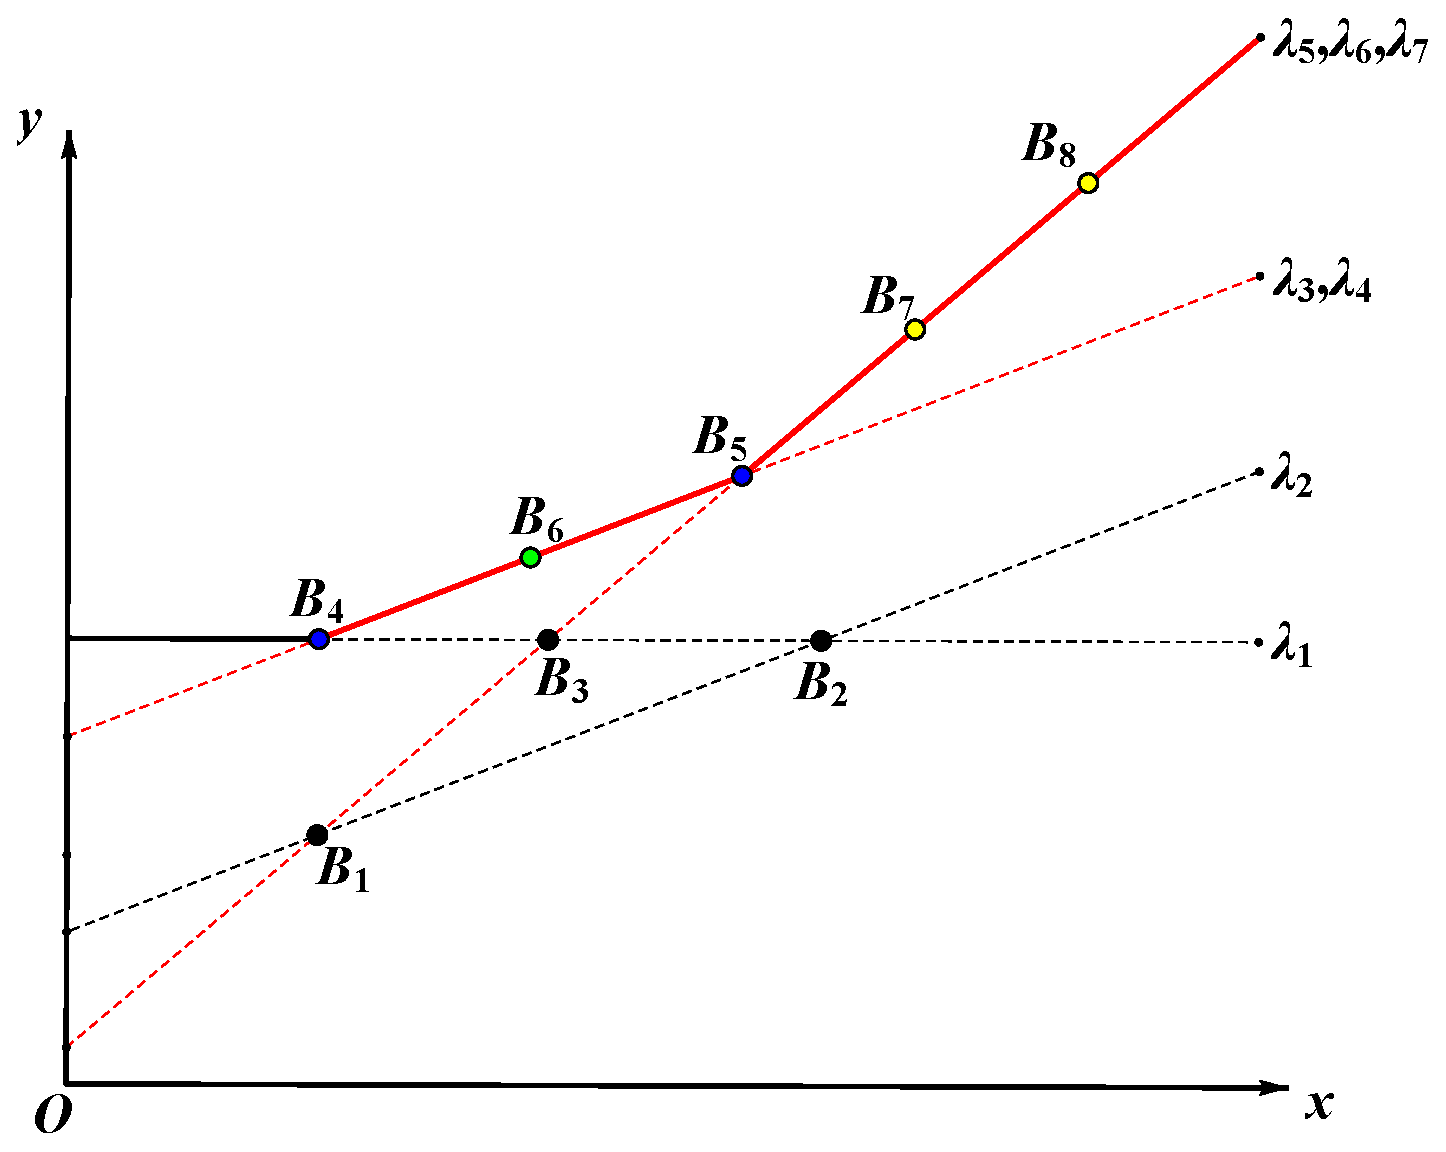
\includegraphics[width=0.6\textwidth]{fig/ps.eps}
\caption{平衡点分类示意图}
\label{point}
\end{figure}
\begin{compactitem}[\textbullet]
\item 尽管$B_1,B_2,B_3$是不同直线的交点, 但是因为它们不满足最大性约束, 所以他们不是平衡点. 
\item 而$B_4,B_5$ 是不同直线的交点且满足最大性约束, 所以它们是第一类平衡点.
\item $B_6$虽然不是不同直线的交点, 但有多条直线穿过它. 又因为它在$B_4$ 和 $B_5$ 之间, 所以它是第二类平衡点.
\item $B_7,B_8$以及它们右侧的更多整点是可能的第三类平衡点\BPthree{}. 因为有多条重复直线穿过它们, 且它们的右侧没有其它直线的交点. 我们可以通过$n$阶展开方法来确定这一类平衡点的上界.
\end{compactitem}

接着, 我们将给出一些具有代表性的例子. 

\begin{example}
(\BPone{})
\begin{equation}
-x^4f(x+3)+(x+1)f(x)^2+8x^6+27x^5+28x^4+2x^3-x-1=0 \label{ep1} .
\end{equation}

我们可以得到其次数列表为$[m+4,2m+1,6]$. 因为没有重复的次数, 所以该方程只有\BPone{}. 从 $m+4=6,2m+1=6$ 和 $m+4=2m+1$ 可以得出 $M_1=\{2,3\}$, 从而$\overline m = 3$. 然后, 将$f(x)=\sum\nolimits_{k=0}^3{\mu_k x^k}$ 代入原方程, 我们可以得到如下方程组:
\begin{equation}
\left\{
\begin{array}{l}
    {\mu_{{0}}}^{2}-1=0,                                                                                                  \\
    {\mu_{{3}}}^{2}-\mu_{{3}}=0,                                                                                            \\
    {\mu_{{0}}}^{2}+2\,\mu_{{0}}\mu_{{1}}-1=0,                                                                                \\
    2\,\mu_{{0}}\mu_{{1}}+2\,\mu_{{0}}\mu_{{2}}+{\mu_{{1}}}^{2}=0,                                                                \\
    2\,\mu_{{2}}\mu_{{3}}+{\mu_{{3}}}^{2}-\mu_{{2}}-9\,\mu_{{3}}+8=0,                                                             \\
    2\,\mu_{{0}}\mu_{{2}}+2\,\mu_{{0}}\mu_{{3}}+{\mu_{{1}}}^{2}+2\,\mu_{{1}}\mu_{{2}}+2=0,                                            \\
    2\,\mu_{{1}}\mu_{{3}}+{\mu_{{2}}}^{2}+2\,\mu_{{2}}\mu_{{3}}-\mu_{{1}}-6\,\mu_{{2}}-27\,\mu_{{3}}+27=0,                              \\
    2\,\mu_{{0}}\mu_{{3}}+2\,\mu_{{1}}\mu_{{2}}+2\,\mu_{{1}}\mu_{{3}}+{\mu_{{2}}}^{2}-\mu_{{0}}-3\,\mu_{{1}}-9\,\mu_{{2}}-27\,\mu_{{3}}+28=0.
\end{array}
\right.
\label{ceqs}
\end{equation}
可以解得, \refeqnn{ceqs}的解为$\{\mu_0=-1,\mu_1=0,\mu_2=0,\mu_3=1\}$. 最终我们得到, \refeqnn{ep1}的多项式解为$f(x)=x^3-1$.
\end{example}

\begin{example}
(\BPtwo{})
\begin{equation}
x^2f(x)f(x+1)f(x+2)+(1-x^9)f(x)+(x^4-x^9)f(x+1)+2x^9f(x+2)-\sum_{k=0}^{10}{c_k x^k}=0, \label{ep2}
\end{equation}
其中$[c_0,\cdots,c_{10}]=[1,1,22,57,85,72,35,9,1,10,6]$. 该方程的次数列表为$[3m+2,m+9,m+9,m+9,10]$. 从$m+9=10$可以得到第一类平衡点$M_1=\{1\}$. 因为$m+9$有两个, 且它关于$m$的系数不是最大的, 所以该方程有\BPtwo{}. 从$\{m+9> 10,m+9> 3m+2\}$可以得出$m< 7/2$. 因此, $\overline m=3$. 然后, 可以解得原方程的多项式解为$f(x)=x^2+x+1$. 显然, 如果不考虑\BPtwo{}, 我们将无法得到该方程的多项式解. 
\end{example}

\begin{example} \label{examp-3}
(\BPthree{}, 2阶展开)
\begin{equation}
(x+2)f(x)-(x-1)f(x+1)=0. \label{ep3}
\end{equation}
因为该方程的次数列表为$[m+1,m+1]$, 所以它只有\BPthree{}. 基于2阶展开, 即将$f(x)=u_0 x^m + u_1 x^{m-1} + \OO(x^{m-2})$ 代入到原方程中, 可以得到
\begin{equation}
(-u_0 m+3u_0)x^m+\OO(x^{m-1})=0.
\end{equation}
从 $-u_0 m+3u_0=0$ 可以解得 $m=3$. 然后, 基于待定系数法可以可以解得该方程的多项式为 $f(x)=c(x^3-x)$, 其中 $c$ 是任意常数.
\end{example}

\begin{example}
(\BPthree{}, 高阶展开)
\begin{equation}
-2x^5f(x)f(x+2)+x^4f(x)^2+(2x^5-x^4)f(x+1)^2-\sum_{k=0}^{22}{c_k x^k}=0, \label{ep4}
\end{equation}
其中 $[c_0,\cdots,c_{22}]=$[0, 0, 0, 0, 1, 2046, 10140, 22340, 28095, 20730, 7788, 6120, 30600, 84180, 151164, 199504, 199710, 151380, 85560, 35136, 10035, 1830, 170]. 该方程的次数列表为 $[2m+5,2m+4,2m+5,22]$. 由 $2m+5=22$ 可得 $ m=17/2$, 该方程没有\BPone{}. 所以该方程只有\BPthree{}. 该方程的$n$阶展开中的第一个非零项为 
\begin{equation}
\Omega_3 = 2m^2u_0^2-3mu_0^2-2u_0u_1.
\end{equation}
因为$\Omega_3=0$关于$m$没有正整数解, 所以当$\Omega_3$有效方程没有多项式解. 换句话说, 只有$2m+5>22+3$不成立, 即$m\le 10$时, 才有多项式解. 从而, $\overline m =10$, 可以得到\refeqnn{ep4} 的多项式解为 $f(x)=\pm (x^{10}-1)$.
\end{example}

\begin{example}
(应用, 2阶展开)

为了计算 
\begin{equation}
    S(x)=\sum_{k=0}^x{k^{10}}
\end{equation}
的闭形式解, 我们可以构造差分方程
\begin{equation}
    S(x)-S(x-1)=x^{10}, S(0)=0. \label{seq}
\end{equation}
该方程的次数列表为$\mbrace{m,m,10}$. 此时, $m=10$ 是 \BPone{}. 因为这里有两个重复的$m$, 所以我们需要考虑\BPthree{}. 该方程的二阶展开为
\begin{equation}
u_0m x^{m-1}+\OO(x^{m-2})=0.   
\end{equation}
因为当$m-1>10$时, $\Omega_1=u_0m$有效, 方程没有多项式解. 所以, 必须有$m\le 11$. 从而, $\overline m=11$. 我们可以得到原方程的多项式解为
\begin{equation}
S(x)=\frac{5}{66}x-\frac{1}{2}x^3+x^5-x^7+\frac{5}{6}x^9+\frac{1}{2}x^{10}+\frac{1}{11}x^{11}.
\end{equation}
从这个例子中也可以看出, 如果不考虑第三类平衡点, 我们也不能得到多项式解. 

另一方面, 因为\refeqnn{seq}是一个线性方程, 它能够被其它方法求解, 例如\citett{Abramov1989polynomial} 和\citett{Abramov1995polynomial} 中的方法. 但是, 这个方程在我们的方法中是通过2阶展开进行求解的, 这也说明$n$阶展开方法在我们的算法中是至关重要的.  
\end{example}

\begin{example}
(应用, logistic方程, 也称虫口方程)

因为我们的算法能够找到所有的多项式解, 所以如果我们的算法没有解则表示方程没有多项式解. 考虑著名的logistic 方程\citep{may1976simple}
\begin{equation}
    f(x+1)=r f(x)\sbrace{1-f(x)},
\end{equation}
其中 $r$ 是一个常数. 该方程的阶数列表为 $\mbrace{2m,m,m}$. 因为 $2m\ge m$, 所以该方程只有\BPone{}, 即$2m=m\Rightarrow m=0$. 最终我们可以的得出, 该方程除了$f(x)=0$和$f(x)=(r-1)/r$以外, 没有其它非平凡的多项式解.
\end{example}

\begin{example}
(应用, Riccati方程)

对于 Riccati 方程\citep{bittanti2012riccati}
\begin{equation}
    f(x+1)f(x)+A(x)f(x)+B(x)f(x+1)=C(x), \label{raeq}
\end{equation} 
其中$A(x),B(x)$ 和 $C(x)$ 是多项式系数. 例如取
\begin{equation}
\begin{split}
A(x)&= -\frac{1}{2}\sbrace{x^5+5x^4-40x^2-2}, \\ 
B(x)&= -\frac{1}{2}\sbrace{x^5+10x^3-x-2}, \\ 
C(x)&= -x\sbrace{x+1}\sbrace{48x^4+20x^2-5x-3}.
\end{split}
\end{equation}
则该方程的次数列表为$\mbrace{2m,m+5,m+5,6}$. 对于平衡点的分类讨论如\reftab{tb}所示.

\begin{table}[H]
\centering
\caption{平衡点的分类讨论}\label{tb}
\begin{tabular}{ccc}
\hline
平衡点类型 & 平衡方程 & 平衡点  \\ 
\hline
\BPone{}  & $2m=m+5\ge 6$            & $m=5$             \\ 
\BPone{}  & $2m=6\ge m+5$            & $m\in \varnothing$             \\ 
\BPone{}  & $m+5=6\ge 2m$            & $m=1$             \\ 
\BPtwo{}  & $m+5>\max\bbrace{2m,6}$  & $m\in \bbrace{2,3,4}$ \\
\hline
\end{tabular}
\end{table}
从\reftab{tb}中可以得出$M_1=\bbrace{1,5},M_2=\bbrace{2,3,4}$. 因此, $\overline m=5$. 最终我们可以得到该方程的多项式解为$f(x)=x^5-x$. 

在 Maple 中, 使用 \cd{rsolve} 求解 \refeqnn{raeq} 会得到
\begin{equation}
\begin{split}
    &f(x)=(f \left( 0 \right) \alpha(x)\,{x}^{5}+f \left( 0 \right) \beta(x)\,{x}^{5}+10\,f \left( 0 \right) \alpha(x)\,{x}^{3}-10\,f \left( 0 \right) \beta(x)\,{x}^{3}+2\,{x}^{5}\\
    &-f \left( 0 \right) \alpha(x)\,x-f \left( 0 \right) \beta(x)\,x-2\,f \left( 0 \right) \alpha(x)+2\,f \left( 0 \right) \beta(x)-2\,x)/(2+2f(0)\alpha(x)) . 
\end{split} \label{rasol_real}
\end{equation}
其中,
\begin{equation}
\begin{split}
&\alpha(x)=\sum_{k_1=0}^{x-1}\mbrace{
    \frac{(-1)^{k_1}p(k_1)}{q(k_1)}\prod_{k_0=0}^{k_1}{
        \frac{q(k_0)}{p(k_0)}
    }
}, \\
&\beta(x)=\sum_{k_1=0}^{x}\mbrace{
    \frac{(-1)^{k_1}p(k_1)}{q(k_1)}\prod_{k_0=0}^{k_1}{
        \frac{q(k_0)}{p(k_0)}
    }
}, \\
&p(x)=x^5+5x^4-20x^2-26x+8, \\
&q(x)=x^5+5x^4+20x^3+10x^2+8x+2. 
\end{split}
\end{equation}
将 $f(0)=0$ 代入\refeqn{rasol_real}, 可以得到 $f(x)=x^5-x$. 这表示该多项式解释在初始条件 $f(0)=0$ 下的解. 此外, 需要注意的是, 使用 \cd{LRETools[riccati]} 来求解\refeqnn{raeq}将得到错误的解, 这显然是该函数的一个BUG. 
\end{example}

\section{NEM软件包的实现}
在上文中, 我们以差分方程多项式解为例, 展示了$n$阶展开方法的作用. 实时上, $n$阶展开方法也能用于完善其它基于齐次平衡原则方法. 为了能够更加方便的将$n$阶展开方法应用到相关问题中去, 本文决定将$n$阶展开方法单独实现为一个\cd{NEM}软件包.

从上文的分析可以看出, 在计算\BPone{}和\BPtwo{}时, 只需要关注方程的各项次数, 而计算\BPthree{}则需要借助于$n$阶展开多项式来计算最高$n$的系数. 事实上, 只要列出了$n$阶展开多项式, 也能获得方程各项的次数. 因此, 我们将$n$阶展开多项式作为\cd{NEM}的输入对象. 在应用到具体问题时, 只需将对应问题中的各项转化为$n$阶展开多项式, 就能调用\cd{NEM}来确定平衡带点的上界, 后续的求解也交给对应问题的相关程序进行解决. 

在\cd{NEM}软件包中, 我们将将$n$阶展开多项式实现为\cd{NEPoly}对象. \cd{NEPoly}对象有三个关键属性: $p,q$和$u$. 其中, $pm+q$就是该多项式的次数, 而$u$则是最高$n$项的系数. 并且, \cd{NEPoly}对象还根据\refeqn{NEM-shift}\D \refeqn{NEM-times} 和 \refeqn{NEM-add} 分别实现了移位\D 乘法和加法操作. 此外, 为了能够将程序应用到微分方程求解的相关问题中去, 我们还推导了微分的计算规则:
\begin{equation}
\begin{split}
& \DIF{t}F\sbrace{x,m,u\up{n}}  \\
=& \DIF{t}\sbrace{\sum_{k=0}^{n-1}{u_k x^{m-k}}+\OO(x^{m-n})} \\
=& \sum_{k=0}^{n-1}{\DIFF{u_k}{t}x^{m-k}}+\DIFF{x}{t}\cdot\sum_{k=0}^{n-1}{u_k (m-k) x^{m-k-1}}+\DIFF{x}{t}\cdot\OO(x^{m-n-1}) \\
=& \sum_{k=0}^{n-1}{\DIFF{u_k}{t}x^{m-k}}+\DIFF{x}{t}\cdot\sbrace{\sum_{k=0}^{n-1}{u_k (m-k) x^{(m-1)-k}}+\OO\sbrace{x^{(m-1)-n)}}} \\ 
=& F\sbrace{x,m,v\up{n}}+\DIFF{x}{t}\cdot F\sbrace{x,m-1,w\up{n}}.
\end{split}\label{NEM-diff}
\end{equation}
其中, 
\begin{equation}
v_p=\DIFF{u_p}{t}, w_p=u_p(m-p).
\end{equation}
只需将$\DIFF{x}{t}$也表示成关于$x$的$n$阶展开多项式, 就能使得\cd{NEPoly}关于导数的计算结果也是$n$阶展开多项式. 

在实现了\cd{NEPoly}之后, 我们实现了\cd{NEM}的核心接口\cd{nem(vs)}, 其中\cd{vs}是一个\cd{NEPoly}列表, 表示方程中各个加法项转化为$n$阶展开多项式的结果. \cd{nem(vs)}的核心逻辑如\refalg{nem}所示. 

\begin{algorithm}
\newcommand{\kw}[1]{\mathbf{~#1~}}
\newcommand{\Fcn}[1]{\mathtt{#1}}
\renewcommand{\lfrac}[2]{\sbrace{#1}/\sbrace{#2}}
\caption{NEM 核心算法 \cd{nem(vs)}}\label{nem}
\KwIn{\cd{NEPoly}对象的列表.}
\KwOut{平衡点上界, $-\infty$ 表示没有找到平衡点.}
$s,d,\sigma,\delta,l\gets \Fcn{getOrders}(vs)$\tcp*[r]{从输入对象中获取相关次数}
$m_1,m_2,m_3\gets -\infty$\tcp*[r]{初始化三种类型平衡点的上界.}
$needBP3\gets\kw{false}$\tcp*[r]{用于记录是否需要 \BPthree{}.}
\For{$i \kw{from} 1 \kw{to} l$}{\label{for-1-start}
    \For{$j \kw{from} i+1 \kw{to} l$}{
        \uIf(\tcp*[f]{寻找 \BPone{}.}){$s_i\neq s_j$}{
            $m\gets (d_j-d_i)/(s_i-s_j)$\;
            \If{$m\in \mathbb Z_+ \kw{and} s_im+d_i\ge \max\{s_km+d_k\}$}{
                $m_1\gets \max(m,m_1)$\;
            }
        }\ElseIf(\tcp*[f]{寻找 \BPtwo{}.}){$s_i=s_j \kw{and} d_i=d_j$}{
            \If(\tcp*[f]{判定是否需要\BPthree{}.}){$s_i=\sigma \kw{and} d_i=\delta$}{
                $needBP3\gets \kw{true}$;~\textbf{continue}\;
            }
            $lb\gets \floor{\underset{s_i>s_k}{\max}{\lfrac{d_k-d_i}{s_i-s_k}}}+1$\;
            $ub\gets \ceil{\underset{s_i<s_k}{\min}{\lfrac{d_k-d_i}{s_i-s_k}}}-1$\;
            \If{$ub\neq +\infty \kw{and} lb\le ub \kw{and} ub\ge 0$}{
                $m_2\gets \max(ub,m_2)$\;
            }
        }
    }
}\label{for-1-end}
\If(\tcp*[f]{寻找 \BPthree{}.}){$needBP3$}{
    $r\gets \sum_{v\in vs}{v}$;~$\Omega\gets r.u$\; \label{add-nem}
    \For{$k \kw{from} 0 \kw{to} n-1$}{\label{for-2-start}
        \If{$\Omega_k\neq 0$}{
            $sol\gets \Fcn{solve}(\Omega_k=0,m)$\;
            $m_{31}\gets \max(sol \bigcap \mathbb{Z}_+)$\tcp*[r]{有解时的上界}
            $m_{32}\gets \floor{\underset{s_j<\sigma}{\max}{\lfrac{d_j-\delta+k}{\sigma-s_j}}}$\tcp*[r]{无解时的上界}
            $m_3\gets \max(m_{31},m_{32})$\;
            \textbf{break}\;
        }
    }\label{for-2-end}
    \If{$m_3=-\infty$}{
        \cd{warning}(`$n$ need be increased.')\;
    }
}
\Return{$\overline m= \max(m_1,m_2,m_3)$}\;
\end{algorithm}

在\refalg{nem}中, 我们首先按照前文的定义, 从\cd{NEPoly}对象中提取相关次数. 然后, 在\refcln{for-1-start}到\refcln{for-1-end}中, 基于这些次数寻找\BPone{}和\BPtwo{}. 在此过程中, 我们也会检测当前问题是否需要继续寻找\BPthree{}. 因为在这个过程中, 我们需要对$l$个输入项进行两两比较, 在内部的计算中也需要寻找这$l$个对象中的相关最值, 所以, 这个过程的时间复杂度为$\OC(l^3)$.

若需要继续计算\BPthree{}, 我们则会在\refcln{add-nem}中对输入的\cd{NEPoly}对象求和, 然后在 \refcln{for-2-start} 到 \refcln{for-2-end} 中寻找\BPthree{}. 这里, $m_{31}$是第一个非零系数等于零关于$m$有解时\BPthree{}的上界, 而$m_{32}$则是无解时的上界. 因为这两者在其中一个有非负值时, 另一个必然为$-\infty$, 所以可以取两者的最大值来确定\BPthree{}的上界. 事实上, $m_{31}$和$m_{32}$分别对应了\refeqn{BP31}和\refeqn{BP32}. 此外, 如果在当前$n$项中并未找到非零系数, 则程序会提醒用户增大展开阶数继续尝试. 在这一部分, 程序首先对$l$个输入项求和, 这部分时间复杂度为$\OC(nl)$. 然后, 程序要在$n$个展开项中寻找非零项, 找到之后需要计算$l$个输入项的最值, 不考虑求解方程的复杂, 则其时间复杂度为$\OC(n+l)$.

最后, 取三类平衡点的最大值就能确定平衡点的上界. 最终, \refalg{nem}的时间复杂度为$\OC(l^3+nl+n+l)$. 当$n$没有远大于$l$时, 时间复杂度等价于$\OC(l^3)$.

\section{NLREPS软件包的实现与测试}
基于\cd{NEM}, 我们能够很方便的实现求解非线性差分方程多项式解的软件包\cd{NLREPS}.
\begin{compactenum}[(1)]
\item 首先, 我们对于形如\refeqn{eq}的输入方程, 将各项系数$a_k(x)$用\refeqn{nepoly-a}转化为\cd{NEPoly}对象, 将未知函数$f(x)$按照\refeqn{nepoly-f}转化为\cd{NEPoly}对象. 
\item 然后, 调用\cd{NEPoly}的内置功能, 基于\refeqn{NEM-shift}计算移位, 基于\refeqn{NEM-times}计算乘法, 得到各个加法项对应的\cd{NEPoly}对象. 
\item 接着, 通过调用\refalg{nem}所对应\cd{nem}函数, 计算平衡点的上界$\overline{m}$.
\item 最后, 用待定系数法, 将$f(x)=\sum_{k=0}^{\overline{m}}{\mu_k x^k}$代入原方程求解即可. 
\end{compactenum}

按照上述方法, 我们实现了\cd{NLREPS}, 其核心接口为
\begin{verbatim}
nlreps(eq,fx,{nExpand,inits}).
\end{verbatim}
其中,
\begin{compactitem}[\textbullet]
\item \cd{eq} 是输入的方程.
\item \cd{fx} 是需要求解的未知函数, 如$f(x)$.
\item \cd{nExpand} 表示展开阶数. 这个参数是可选的, 默认值为\cd{nExpand=5}. 
\item \cd{inits} 表示初始条件, 例如 \cd{\{f(0)=0, f(1)=1\}}. 这个参数也是可选的, 默认为空集, 表示没有初始条件. 
\end{compactitem}

例如, 对于\refeg{examp-3}中的问题, 若添加初始条件$\{f(0)=-1\}$, 并指定求解时展开阶数为4, 则调用方式为
\begin{verbatim}
nlreps(eq,f(x),nExpand=4,inits={f(0)=-1});
\end{verbatim}
然后, 我们就能得到解 $\{f(x)=x^{10}-1\}$.

为了测试\cd{NLREPS}的求解性能, 我们随机生成了1000个不同规模的问题进行测试. 我们产生测试用例的方法如下.

我们将 
\begin{equation}
    F=\sum_{k=0}^l{\mbrace{a_k(x)\prod_{i=0}^r{f^{\gamma_{ki}}(x+i)}}}
\end{equation}
看作是关于$f(x),\cdots,f(x+r)$的多元多项式, 其系数为 $a_k(x)$. 对于这个多项式, 我们取
\begin{equation}
\begin{split}
&\max{\rm deg}(a_k(x))=\max d_k=10,\\ 
&\max{\rm deg}(F)=\max s_k=5, \\
&l\in [2,400], r=5.
\end{split}
\end{equation}
生成$F$之后,我们生成一个随机的解$f^*(x)$代入$F$得到$g(x)$, 最终得到方程$F-g(x)=0$. 其中, ${\rm deg}(f^*(x))\le 10$. 生成1000个测试用例之后, 我们从3个方面对它们进行分析. 

首先, 我们考虑测试\cd{nlreps}的运行时间. 因为求解代数方程组并不是\cd{NLREPS}的主要职责, 所以我们只计算\cd{nem}的运行时间. 我们取展开阶数为5进行测试, 所得结果如\reffig{t-nem}所示. 从\reffig{t-nem}中可以看出, 运行时间关于输入规模的增长是多项式的, 这符合前文中的理论分析. 
\begin{figure}[htbp]
\centering
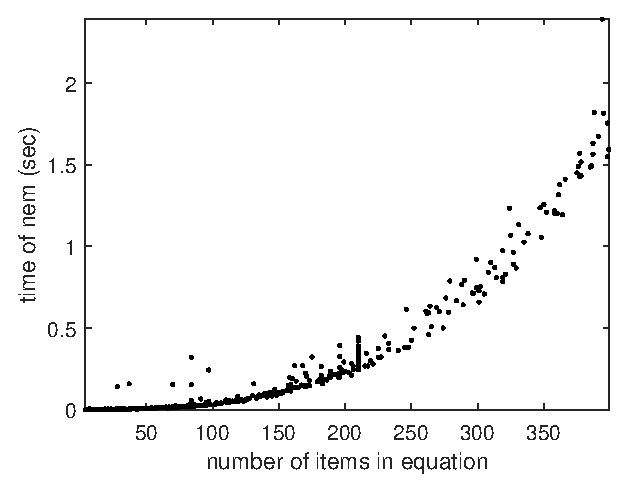
\includegraphics[width=\figwidth]{fig/t-nem.eps}
\caption{NEM 的时间复杂度}
\label{t-nem}
\end{figure}

然后, 我们来关注平衡点类型的分布. 因为一共有三种平衡点, 所以我们用一个长度为3的二进制序列来表示一个方程的平衡点类型. 例如\cd{100}表示只有\BPone{}. 从\reffig{d-bps}可以看出, 几乎每个方程都有\BPone{}, 大部分方程在具有\BPone{}的同时还具有\BPthree{}. 在我们的测试中, 有2个方程只有\BPthree{}, 没有一个方程有\BPtwo{}.
\begin{figure}[htbp]
\centering
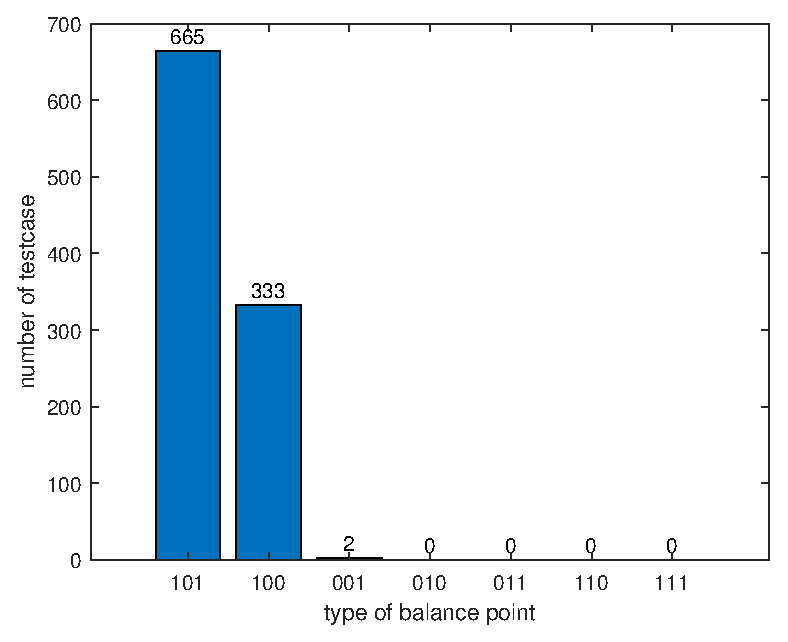
\includegraphics[width=\figwidth]{fig/d-bpType.eps}
\caption{平衡类型分布}
\label{d-bps}
\end{figure}

最后, 我们来关注一下方程的最小展开阶数. 方程的最小展开阶数表示的是方程在展开后第一个非零系数出现的位置. 从\reffig{d-nExpand}中可以看出, 在我们的测试中, 只有2个例子需要二阶展开. 事实上, 这两个方程恰好是那两个只有\BPthree{}的方程. 这说明较小的展开阶数就能解决大部分的问题. 
\begin{figure}[htbp]
\centering
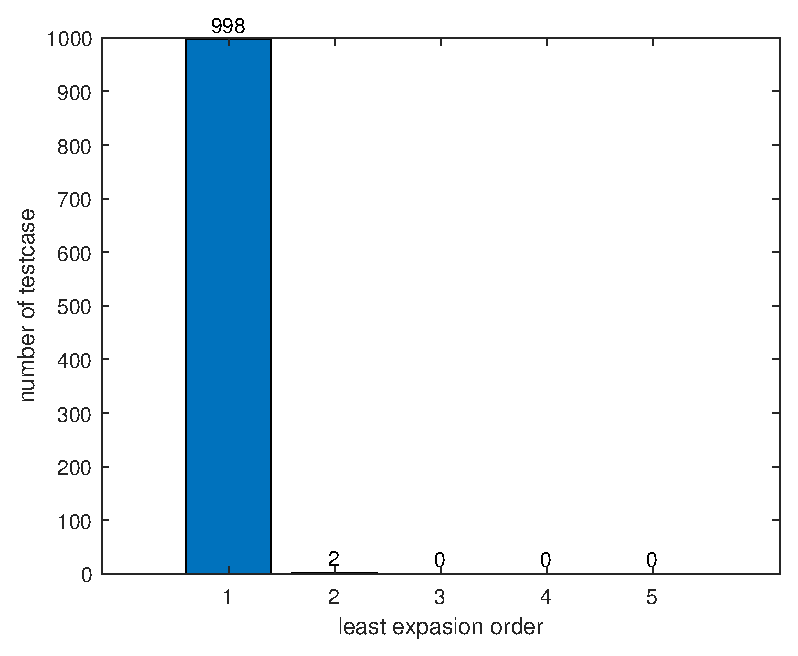
\includegraphics[width=\figwidth]{fig/d-nExpand.eps}
\caption{展开阶数分布}
\label{d-nExpand}
\end{figure}

\section{小结}

在本章中, 我们提出了$n$阶展开方法来完善齐次平衡原则, 并将其应用于非线性差分方程多项式解的求解. 我们针对$n$阶展开方法开发了\cd{NEM}, 并在此基础上开发了求解非线性差分方程多项式解的软件包\cd{NLREPS}. 
